\documentclass[12pt]{report}

\usepackage[english,russian]{babel} 
\usepackage{fontspec} 
\defaultfontfeatures{Ligatures={TeX},Renderer=Basic} 
\setmainfont[Ligatures={TeX,Historic}]{Times New Roman}
\usepackage[utf8]{inputenc}
\usepackage[14pt]{extsizes}
\usepackage{graphicx}
\usepackage{geometry}
\usepackage{listings}
\usepackage{fontspec} 
\usepackage{hyperref}
\usepackage{amsmath,amsfonts,amssymb,amsthm} 
% Для измененных титулов глав:
\usepackage{titlesec, blindtext, color} % подключаем нужные пакеты
\usepackage{setspace} % полуторный интервал
\definecolor{gray75}{gray}{0.75} % определяем цвет
\newcommand{\hsp}{\hspace{20pt}} % длина линии в 20pt
% titleformat определяет стиль
\titleformat{\chapter}[hang]{\Huge\bfseries}{\thechapter\hsp\textcolor{gray75}{|}\hsp}{0pt}{\Huge\bfseries}
\usepackage{caption} % подписи к рисункам в русской типографской традиции

\geometry{top=2cm} % отступ сверху
\geometry{bottom=2cm} % отступ снизу
\geometry{left=3cm} % отступ справа
\geometry{right=1cm} % отступ слева


 \captionsetup[figure]{labelsep=endash,justification=centering,singlelinecheck=false,font=normalsize}

% Для листинга кода:
\lstset{ %
	language=c++,                 % выбор языка для подсветки (здесь это С)
	basicstyle=\small\sffamily, % размер и начертание шрифта для подсветки кода
	numbers=left,               % где поставить нумерацию строк (слева\справа)
	numberstyle=\tiny,           % размер шрифта для номеров строк
	stepnumber=1,                   % размер шага между двумя номерами строк
	numbersep=5pt,                % как далеко отстоят номера строк от подсвечиваемого кода
	showspaces=false,            % показывать или нет пробелы специальными отступами
	showstringspaces=false,      % показывать или нет пробелы в строках
	showtabs=false,             % показывать или нет табуляцию в строках
	frame=single,              % рисовать рамку вокруг кода
	tabsize=2,                 % размер табуляции по умолчанию равен 2 пробелам
	captionpos=t,              % позиция заголовка вверху [t] или внизу [b] 
	breaklines=true,           % автоматически переносить строки (да\нет)
	breakatwhitespace=false, % переносить строки только если есть пробел
	escapeinside={\#*}{*)}   % если нужно добавить комментарии в коде
}


%для графиков
\usepackage{pgfplots}
\usepackage{filecontents}
\usetikzlibrary{datavisualization}
\usetikzlibrary{datavisualization.formats.functions}
\begin{filecontents}{LevTable.dat}
	5 80
	10 120
	50 760
	100 2500
	200 9500
	500 55000
\end{filecontents}

\begin{filecontents}{LevRec.dat}
	5 370
	10 1610000
\end{filecontents}

\begin{filecontents}{LevRecTable.dat}
	5 100
	10 150
	50 1680
	100 6700
	200 25000
	500 160000
\end{filecontents}

\begin{filecontents}{DamLevTable.dat}
	5 80
	10 120
	50 860
	100 2900
	200 11000
	500 65000
\end{filecontents}



\begin{document}	
	%\def\chaptername{} % убирает "Глава"
	\begin{table}[ht]
		\centering
		\begin{tabular}{|c|p{400pt}|} 
			\hline
			\begin{tabular}[c]{@{}c@{}} 
\includegraphics[scale=0.37]{EmblemBMSTU} \\\end{tabular} &
			\footnotesize\begin{tabular}[c]{@{}c@{}}\textbf{Министерство~науки~и~высшего~образования~Российской~Федерации}\\\textbf{Федеральное~государственное~бюджетное~образовательное~учреждение}\\\textbf{~высшего~образования}\\\textbf{«Московский~государственный~технический~университет}\\\textbf{имени~Н.Э.~Баумана}\\\textbf{(национальный~исследовательский~университет)»}\\\textbf{(МГТУ~им.~Н.Э.~Баумана)}\\\end{tabular}  \\
			\hline
		\end{tabular}
	\end{table}
	\noindent\rule{\textwidth}{4pt}
	\noindent\rule[14pt]{\textwidth}{1pt}
	\hfill 
	\noindent
	\makebox{ФАКУЛЬТЕТ~}%
	\makebox[\textwidth][l]{\underline{~~~~«Информатика и системы управления»~~~~~~~~~~~~~~~~~~~~~~~~~~~~~~~~~~~~~~~~~~~~}}%
	\\
	\noindent
	\makebox{КАФЕДРА~}%
	\makebox[\textwidth][l]{\underline{~~~~~~~«Программное обеспечение ЭВМ и информационные технологии»~~~~~~~~}}%
	\\
	
	
	\begin{center}
		\vspace{3cm}
		{\bf\huge Отчёт\par}
		{\bf\Large по лабораторной работе № 2\par}
		\vspace{0.5cm}
	\end{center}
	
	
	\noindent
	\makebox{\large{\bf Название:}~~~}
	\makebox[\textwidth][l]{\large\underline{~Алгоритмы умножения матриц~~~~~~~~~~~~~}}\\
	
	\noindent
	\makebox{\large{\bf Дисциплина:}~~~}
	\makebox[\textwidth][l]{\large\underline{~Анализ алгоритмов~~~~~~~~~~~~~~~~~~~~~~~~~~~~~~~~~~~~~~~~~~~~~~~~~~~~}}\\
	
	\vspace{1.5cm}
	\noindent
	\begin{tabular}{l c c c c c}
		Студент      & ~ИУ7-55Б~               & \hspace{3.5cm} & \hspace{3.5cm}                 & &  Д.В. Сусликов \\\cline{2-2}\cline{4-4} \cline{6-6} 
		\hspace{3cm} & {\footnotesize(Группа)} &                & {\footnotesize(Подпись, дата)} & & {\footnotesize(И.О. Фамилия)}
	\end{tabular}
	
	\vspace{1cm}
	
	\noindent
	\begin{tabular}{l c c c c}
		Преподователь & \hspace{6cm}   & \hspace{3.5cm}                 & & Л.Л. Волкова \\\cline{3-3} \cline{5-5} 
		\hspace{3cm}  &                & {\footnotesize(Подпись, дата)} & & {\footnotesize(И.О. Фамилия)}
	\end{tabular}
	
	\begin{center}	
		\vfill
		\large \textit {Москва, 2020 г.}
	\end{center}
	
	\thispagestyle {empty}
	\pagebreak
	
	\tableofcontents
	\onehalfspacing
	
	\newpage
	\chapter*{Введение}
	\addcontentsline{toc}{chapter}{Введение}
	Цель данной лабораторной работы - изучение алгоритмов умножения матрицы, получение навыков улучшения алгоритмов и подсчёта их трудоёмкости. В ходе работы будут рассмотрены 3 алгоритма:
	\begin{enumerate}
		\item[1)] стандартный алгоритм умножения матриц;
		\item[2)] алгоритм Винограда;
		\item[3)] улучшенный алгоритм Винограда.
	\end{enumerate}
	В лабораторной работе требуется:
	\begin{enumerate}
		\item[1)] изучить алгоритмы умножения матриц;
		\item[2)] оптимизировать алгоритм Винограда;
		\item[3)] дать теоритическую оценку стандартного алгоритма умножения матриц, алгоритма Винограда и улучшенного алгоритма Винограда;
		\item[4)] реализовать три алгоритма умножения матриц;
		\item[5)] сравнить алгоритмы умножения матриц.		
	\end{enumerate}
	
	
	\newpage
	\chapter{Аналитическая часть}
	В данном разделе представлены математические описания алгоритмов умножения матриц.
	
	\section{Стандартный алгоритм умножения матриц}
	
	Матрица — математический объект, записываемый в виде прямоугольной таблицы элементов кольца или поля (например, целых, действительных или комплексных чисел), которая представляет собой совокупность строк и столбцов, на пересечении которых находятся её элементы. Количество строк и столбцов задает размер матрицы. Хотя исторически рассматривались, например, треугольные матрицы, в настоящее время говорят исключительно о матрицах прямоугольной формы, так как они являются наиболее удобными и общими. 
	
	Умножение матриц — одна из основных операций над матрицами. Матрица, получаемая в результате операции умножения, называется произведением матриц.
	
	Пусть даны две прямоугольные матрицы А и В размеров $[m * n]$ и $[n * k]$ соответственно.  
	В результате произведение матриц A и B получим матрицу C размера $[m *  k]$.
		\begin{equation}
		c_{i,j} = \sum_{r=1}^{m}a_{ir}b_{rj} \qquad (i=1,2,...l; j = 1,2,...n)
	\end{equation}
	Операция умножения двух матриц выполнима только в том случае, если число столбцов в первой матрице совпадает с числом строк во второй, то эти две матрицы можно перемножить.
	

	\section{Алгоритм Винограда}
	Если посмотреть на результат умножения двух матриц, то видно, что каждый элемент в нем представляет собой скалярное произведение соответствующих строки и столбца исходных матриц. Можно заметить также, что такое умножение допускает предварительную обработку, позволяющую часть работы выполнить заранее. \hyperref[literature]{[1]}\par
	Рассмотрим два вектора $V = (v_{1},v_{2},v_{3},v_{4})$ и $W = (w_{1},w_{2},w_{3},w_{4})$. Их скалярное произведение равно:
	\begin{equation}
		V * W = v_{1}w_{1} + v_{2}w_{2} + v_{3}w_{3} + v_{4}w_{4}
	\end{equation}
	Это равенство можно переписать в виде:
	\begin{equation}
		V * W = (v_{1} + w_{2})(v_{2} + w_{1}) + (v_{3} + w_{4})(v_{4} + w_{3}) -  v_{1}v_{2} - v_{3}v_{4} - w_{1}w_{2} - w_{3}w_{4}
	\end{equation}
	Менее очевидно, что выражение в правой части последнего равенства допускает предварительную обработку: его части можно вычислить заранее и запомнить для каждой строки первой матрицы и для каждого столбца второй. На практике это означает, что над предварительно обработанными элементами придется выполнять лишь первые два умножения и последующие пять сложений, а также дополнительно два сложения. 
	
	\section*{Вывод}
	\addcontentsline{toc}{chapter}{Вывод}
	Таким образом, получилось узнать, что из себя представляет умножение матриц. Были описаны стандартный алгоритм умножения и Винограда, объяснено преимущество второго над первым.
	
	\chapter{Конструкторская часть}
	В данном разделе представлены схемы алгоритмов и дана оценка их трудоемкости.
	
	\section{Схемы алгоритмов}
	Ниже на Рисунке 1 представлена схема стандартного алгоритма умножения матриц.
	\begin{figure}[h!]
		\center{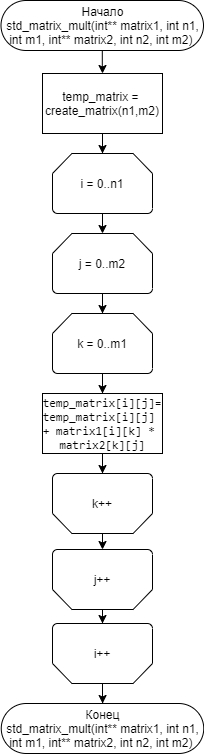
\includegraphics[scale= 0.8]{1.png}}
		\caption*{Рисунок 1 - Схема стандартного алгоритма умножения матриц}
	\end{figure}
	
	\newpage
	Далее на Рисунке 2 можно увидеть схему алгоритма Винограда.
	\begin{figure}[h!]
		\center{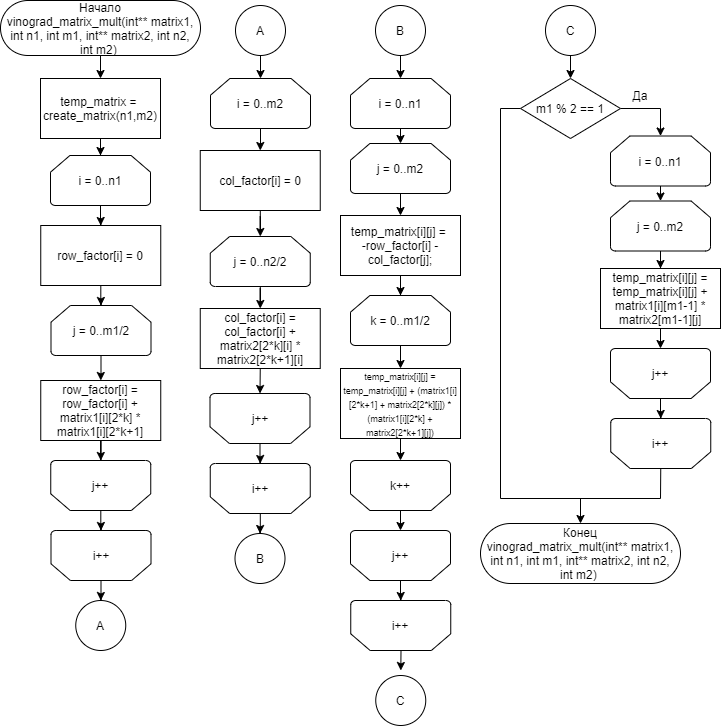
\includegraphics[scale= 0.7]{2.png}}
		\caption*{Рисунок 2 - Схема алгоритма Винограда}
	\end{figure}
	
	
	\newpage
	Ниже на Рисунке 3 показана схема модифицированного алгоритма Винограда.
		\begin{figure}[h!]
		\center{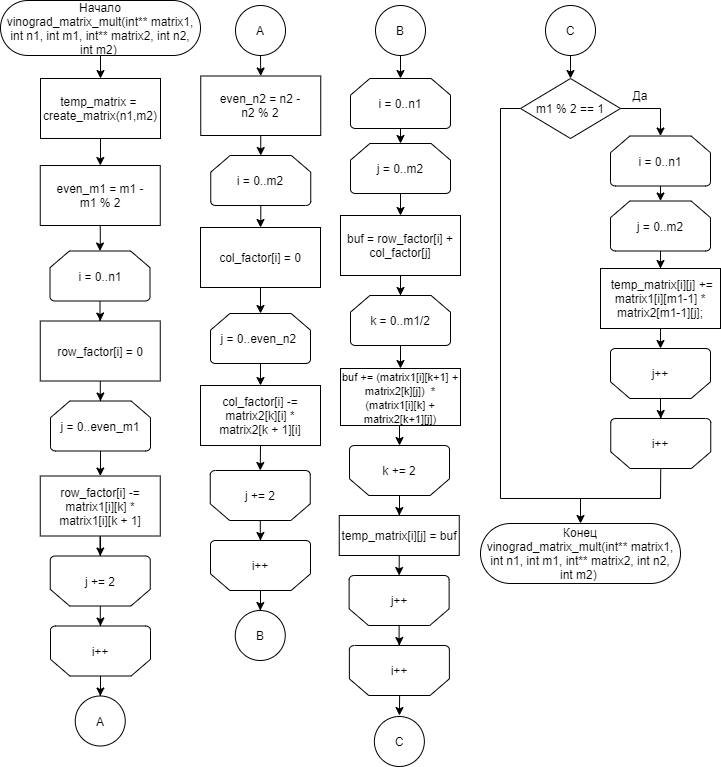
\includegraphics[scale= 0.7]{3.png}}
		\caption*{Рисунок 3 - Схема модифицированного алгоритма Винограда}
	\end{figure}

	\newpage
	\section{Отличие модифицированного алгоритма Винограда от обычного}
	 Улучшения:
	\begin{itemize}
		\item[1)] нет нужды внутри цикла каждый раз пересчитывать $m1 / 2$ и $n2 / 2$, так как заранее посчитано $even\_m1 = m1 - m \% 2$ и $even\_n2 = n2 - n2 \% 2$;
		\item[2)] так как есть $even\_m1$ и $even\_n2$, то индекс будет изменятся на 2 - $j += 2$, следовательно нет нужды умножать на 2, как в обычном алгоритме, где индекс матрицы считался $matrix1[i][2 * j]$;
		\item[3)] в обычном алгоритме значение $-row\_factor[i] - col\_factor[j]$ присваивается элементу матрицы умножения, и в следующем цикле каждый раз происходит обращение к нему. В модифицированном алгоритме Винограда это значение присваивается буферу, и лишь потом после выполнения цикла записывается в матрицу-результат;
		\item[4)] подставлены $+=$ и $-=$, где возможно.
	
	\end{itemize}
	
	
	\section{Трудоемкость алгоритмов}
	Введем модель трудоемкости для оценки алгоритмов: 
	\begin{itemize}
		\item[1)] Операции, чья стоимость 1: $=, +, *, \simeq, <, >, \geq, \leq, ==, !=, [], +=, -=, *=, /=, ++, --$;
		\item[2)] стоимость цикла:\par
		$f_{for}=f_{init}+f_{comp}+M(f_{body}+f_{increment}+f_{comp})$\par
		Пример: $for(i=0,i<M;i++){/* body */}$\par
		Результат: $2 + M(2+f_{body})$;
		\item[3)] стоимость условного оператора\par
		Пусть goto (переход к одной из ветвей) стоит 0, тогда\par
		\begin{displaymath}
			f_{f} = \left\{ \begin{array}{l l}
				min(f_{A},f_{B}), & \textrm{лучший случай}\\
				max(f_{A},f_{B}), & \textrm{худший случай}\\
			\end{array} \right.
		\end{displaymath}
	\end{itemize}
	
	Оценим трудоемкость алгоритмов.
	
	\subsection{Трудоемкость общей первичной проверки}
	Трудоемкость проверки $if ((m1 != n2) || n1 == 0 || n2 == 0) { return; }$   - 5.
	
	\subsection{Трудоемкость стандартного алгоритма умножения}
	Расчёт:\par
	$2 + n_1(2 + 2 + m_2(2 + 3 + 2 + m_1(2 + 11))) = 13n_1m_1m_2 + 7n_1m_2 + 4n_1 + 2$
	
	\subsection{Трудоемкость алгоритма Винограда}
	Расчёт:\par
	Первый цикл: $2 + n_1(2 + 2 + 3 + \frac{m_1}{2}(3 + 12)) = 2 + n_1(7 + \frac{15m_1}{2}) = \frac{15}{2}n_1m_1 + 7n_1 + 2$\par
	Второй цикл: аналогично, $\frac{15}{2}m_2n_2 + 7m_2 + 2$\par
	Третий цикл: $2 + n_1(2 + 2 + m_2(2 + 7 + 3 + \frac{m_1}{2}(3 + 23))) = 13 n_1m_1m_2 + 12n_1m_2 + 4n_1 + 2$\par
	Условие: 
	$\begin{bmatrix}
		2    &&, \text{невыполнение}\\
		15n_1m_2 + 4n_1 + 4 &&, \text{выполнение}\\
	\end{bmatrix} $ 	
	\par
	Результат: $ 13n_1m_1m_2 + \frac{15}{2}n_1m_1 + \frac{15}{2}m_2n_2 + 12n_1m_2 + 7n_1 + 7m_2 + 4n_1 + 6 + 
	\begin{bmatrix}
		2    &&, \text{невыполнение}\\
		15n_1m_2 + 4n_1 + 4 &&, \text{выполнение}\\
	\end{bmatrix} $


	\subsection{Трудоемкость модифицированного алгоритма Винограда}
	Расчёт:\par
	Первый цикл: $3 + 2 + n_1(2 + 2 + 2 + \frac{m_1}{2}(2 + 8)) = 5n_1m_1 + 6n_1 + 5$ \par(3 - на переменную вместо $m_1 / 2$)\par
	Второй цикл: аналогично, $5m_2n_2 + 6m_2 + 5$\par
	Третий цикл: $2 + n_1(2 + 2 + m_2(2 + 4 + 2 + \frac{m_1}{2}(2 + 14) + 3)) = 8n_1m_1m_2 + 11n_1m_2 + 4n_1 + 2$ \par
	Условие:
	$\begin{bmatrix}
		2    &&, \text{невыполнение}\\
		12n_1m_2 + 4n_1 + 4 &&, \text{выполнение}\\
	\end{bmatrix} $
	\par
	Результат: $8n_1m_1m_2 + 5n_1m_1 + 5m_2n_2 + 11n_1m_2 + 6n_1 + 6m_2 + 12 + $\par
	$\begin{bmatrix}
		2    &&, \text{невыполнение}\\
		12n_1m_2 + 4n_1 + 4 &&, \text{выполнение}\\
	\end{bmatrix} $ 

	\section*{Вывод}
	\addcontentsline{toc}{chapter}{Вывод}
	В итоге, код алгоритма умножения матриц Винограда больше, чем у стандартного, но трудоемкость меньше. Так же есть воможность модифицировать алгоритм Винограда, чтоб трудоемкость была еще меньше.
	
	
	\chapter{Технологическая часть}
	В данном разделе даны общие требования к программе, средства реализации и реализация алгоритмов.
	\section{Общие требования}
	\textbf{Требования к вводу:}
	\begin{enumerate}
		\item[1)] вводятся размеры матриц;
		\item[2)] вводятся (или автоматически генерируются) матрицы.
	\end{enumerate}
	\noindent\textbf{Требования к программе:}
	\begin{enumerate}
		\item[1)] при вводе неправильных размеров матриц программа не должна завершаться аварийно;
		\item[2)] должно выполняться корректное умножение матриц.
	\end{enumerate}

	\section{Средства реализации}
	В лабораторной работе был использован язык $C$++\hyperref[CPlusPlus]{[1]}, так как он известен, и на нём было написано множество предыдущих работ.
	
	Среда разработки - $Qt$\hyperref[Cute]{[2]}.
	
	Для замеров процессорного времени была использована функция $clock()$\hyperref[CLOCK]{[3]}.
	\newpage


	\section{Реализация алгоритмов}
	Листинг 1 - Алгоритм стандартного умножения матриц
	\begin{lstlisting}
	void std_matrix_mult(int** matrix1, int n1, int m1,\
	int** matrix2, int n2, int m2)
	{
		if ((m1 != n2) || n1 == 0 || n2 == 0)
		{
			std::cout << "Incorrect matrixes" << std::endl;
			return;
		}
		
		int** temp_matrix = create_matrix(n1, m2);
		
		for (int i = 0; i < n1; i++)
		{
			for (int j = 0; j < m2; j++)
			{
				temp_matrix[i][j] = 0;
				for (int k = 0; k < m1; k++)
				temp_matrix[i][j] = temp_matrix[i][j] + matrix1[i][k] * matrix2[k][j];
			}
		}
		
		print_matrix(temp_matrix, n1, m2);
		delete_matrix(temp_matrix, m1);
	}
	\end{lstlisting}
	\newpage

	Листинг 2 - Алгоритм Винограда
	\begin{lstlisting}
	void vinograd_matrix_mult(int** matrix1, int n1, int m1,\
	int** matrix2, int n2, int m2)
	{
		if ((m1 != n2) || n1 == 0 || n2 == 0)
		{
			std::cout << "Incorrect matrixes" << std::endl;
			return;
		}
		
		int** temp_matrix = create_matrix(n1, m2);
		
		int row_factor[n1];
		for (int i = 0; i < n1; i++)
		{
			row_factor[i] = 0;
			for (int k = 0; k < m1 / 2; k++)
			row_factor[i] = row_factor[i] + matrix1[i][2 * k] * matrix1[i][2 * k + 1];
		}
		
		int col_factor[m2];
		for (int i = 0; i < m2; i++)
		{
			col_factor[i] = 0;
			for (int k = 0; k < n2 / 2; k++)
			col_factor[i] = col_factor[i] + matrix2[2 * k][i] * matrix2[2 * k + 1][i];
		}
		
		for (int i = 0; i < n1; i++)
		{
			for (int j = 0; j < m2; j++)
			{
				temp_matrix[i][j] = -row_factor[i] - col_factor[j];
				for (int k = 0; k < m1 / 2; k++)
				temp_matrix[i][j] = temp_matrix[i][j] + (matrix1[i][2 * k + 1] + matrix2[2 * k][j])
				* (matrix1[i][2 * k] + matrix2[2 * k + 1][j]);
			}
		}
		
		if (m1 % 2 == 1)
		{
			for (int i = 0; i < n1; i++)
			{
				for (int j = 0; j < m2; j++)
				temp_matrix[i][j] = temp_matrix[i][j] + matrix1[i][m1 - 1] * matrix2[m1 - 1][j];
			}
		}
		
		print_matrix(temp_matrix, n1, m2);
		delete_matrix(temp_matrix, m1);
	}
	\end{lstlisting}
	
	Листинг 3 - Модифицированный алгоритм Винограда
	\begin{lstlisting}
	void vinograd_modified_matrix_mult(int** matrix1, int n1, int m1,\
	int** matrix2, int n2, int m2)
	{
		if ((m1 != n2) || n1 == 0 || n2 == 0)
		{
			std::cout << "Incorrect matrixes" << std::endl;
			return;
		}
		
		int** temp_matrix = create_matrix(n1, m2);
		
		int row_factor[n1];
		int even_m1 = m1 - m1 % 2;
		for (int i = 0; i < n1; i++)
		{
			row_factor[i] = 0;
			for (int k = 0; k < even_m1; k += 2)
			row_factor[i] -= matrix1[i][k] * matrix1[i][k + 1];
		}
		
		int col_factor[m2];
		int even_n2 = n2 - n2 % 2;
		for (int i = 0; i < m2; i++)
		{
			col_factor[i] = 0;
			for (int k = 0; k < even_n2; k += 2)
			col_factor[i] -= matrix2[k][i] * matrix2[k + 1][i];
		}
		
		for (int i = 0; i < n1; i++)
		{
			for (int j = 0; j < m2; j++)
			{
				int buf = row_factor[i] + col_factor[j];
				for (int k = 0; k < even_m1; k += 2)
				buf += (matrix1[i][k + 1] + matrix2[k][j])
				* (matrix1[i][k] + matrix2[k + 1][j]);
				
				temp_matrix[i][j] = buf;
			}
		}
		
		if (m1 % 2 == 1)
		{
			for (int i = 0; i < n1; i++)
			{
				for (int j = 0; j < m2; j++)
				temp_matrix[i][j] += matrix1[i][m1 - 1] * matrix2[m1 - 1][j];
			}
		}
		
		print_matrix(temp_matrix, n1, m2);
		delete_matrix(temp_matrix, m1);
	}
	
	\end{lstlisting}
	\newpage
	
	\section*{Вывод}
	\addcontentsline{toc}{section}{Вывод}
	По итогу, написанная программа соотвествует всем описанным выше требованиям, алгоритмы были реализованы на C++, так как данный язык известен, выполнено на нём много прошлых работ. 
	
	
	\chapter{Экспериментальная часть}
	В данном разделе представлены результаты работы программы и приведен анализ времени работы кажого из алгоритмов.
	
	\section{Примеры работы программы}
	На Рисунке 4 представлены меню и ввод матриц.
	\begin{figure}[h]
		\center{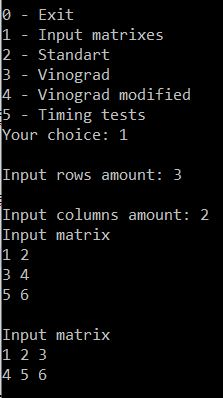
\includegraphics{input.jpg}}
		\caption*{Рисунок 4 - Меню выбора и ввод матриц}
	\end{figure}
	
	\newpage
	На Рисунке 5 изображен результат работы стандартного алгоритма умножения матриц.
	\begin{figure}[h]
		\center{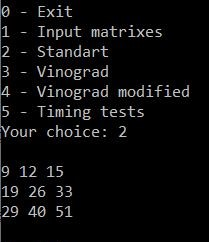
\includegraphics{std.jpg}}
		\caption*{Рисунок 5 - Стандартный алгоритм умножения матриц}
	\end{figure}
	
	
	На Рисунке 6 показан результат работы алгоритма Винограда.
	\begin{figure}[h]
		\center{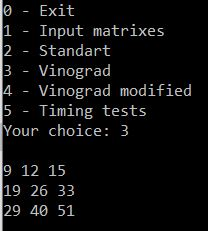
\includegraphics{vin.jpg}}
		\caption*{Рисунок 6 - Алгоритм Винограда}
	\end{figure}
	
	\newpage
	На Рисунке 7 показан результат работы модифицированного алгоритма Винограда.
	\begin{figure}[h]
		\center{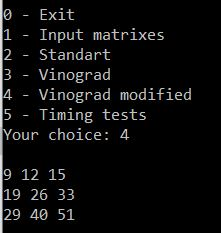
\includegraphics{vinMod.jpg}}
		\caption*{Рисунок 7 - Модифицированный алгоритм Винограда}
	\end{figure}
	
	
	\section{Анализ времени работы алгоритмов }
	Эксперементы проводятся на квадратных матрицах. Элементы матриц задаются случайным образом.\par
	В первом случае размеры матриц: 100х100, 200х200, 300х300, 400х400, 500х500. 
	
	
	
	
	
	
	
	
	
	
	
	\chapter*{Литература}
	\addcontentsline{toc}{chapter}{Литература}
	
	\begin{enumerate}
		\label{CPlusPlus}
		\item[1)] Бьерн Страуструп. Язык программирования С++. -URL:\par 
		\href{https://codernet.ru/books/c_plus/bern_straustrup_yazyk_programmirovaniya_c_specialnoe_izdanie/}
		{https://codernet.ru/books/c\_plus/bern\_straustrup\_yazyk\_programmirovaniya\_
			c\_specialnoe\_izdanie/}\par(дата обращения:
		01.10.2020). Текст: электронный.
		
		\label{Cute}
		\item[2)] Qt. -URL:\par
		\href{https://www.qt.io/}{https://www.qt.io/} (дата обращения: 01.10.2020). Текст: электронный.
		
		\label{CLOCK}
		\item[3)] Функция $clock$. -URL:\par
		\href{https://docs.microsoft.com/ru-ru/cpp/c-runtime-library/reference/clock?view=vs-2019}{https://docs.microsoft.com/ru-ru/cpp/c-runtime-library/reference/clock?view=vs-2019} (дата обращения:
		01.10.2020). Текст: электронный.
		
	\end{enumerate}
	
\end{document}